% Chapter 2
\chapter{مفاهیم پایه در یادگیری فدرال و نگاه کلی به پیشینه پژوهش چالش‌ها}


\section{مقدمه}
توزیع داده‌ها بین کاربران در یادگیری فدرال می‌تواند با چالش‌ها و مشکلات مختلفی مواجه شود. یکی از مسائل مهم، تفاوت‌ها و ناسازگاری‌هایی است که ممکن است در طول فرآیند آموزش بین کاربران یا دستگاه‌های مختلف به وجود بیاید. این اختلافات می‌توانند ناشی از تفاوت در کیفیت داده‌ها، سرعت پردازش یا حتی محیط‌های مختلفی باشند که هر دستگاه در آن قرار دارد. همچنین، تأخیر در ارسال و دریافت داده‌ها بین کاربران و سرور مرکزی نیز می‌تواند چالش دیگری باشد که عملکرد کلی سیستم را تحت تأثیر قرار دهد
\cite{li2020federated}.

اگر این چالش‌ها پیش از آغاز فرآیند مدل‌سازی به درستی شناسایی نشده و راه‌حل‌های مناسبی برای آن‌ها اتخاذ نشود، مدل نهایی احتمالاً با مشکلاتی همچون کاهش دقت و عملکرد روبرو خواهد شد. این مسئله یکی از بزرگترین موانع در مسیر یادگیری فدرال است و نیازمند دقت و استفاده از روش‌های خلاقانه برای حل آن است.

در این فصل، ابتدا به بیان چارچوب ریاضی یادگیری فدرال پرداخته می‌شود که البته برای درک آن نیاز به آشنایی پایه با مفاهیم ریاضی در یادگیری ماشین و یادگیری عمیق است. سپس چالش‌های موجود در یادگیری فدرال بررسی شده و دیدگاه‌های مختلف مقالات علمی در مورد هر یک از این چالش‌ها به صورت کلی مرور می‌شوند. در نهایت، به رویکردهای پایه‌ای جهت حل این چالش‌ها اشاره خواهد شد.


\section{چارچوب ریاضی یادگیری فدرال}
برای تشریح چارچوب ریاضی یادگیری فدرال، ابتدا باید مفاهیم اساسی یادگیری ماشین و یادگیری عمیق را بررسی کرد و رابطه‌های اصلی مرتبط با آن‌ها را بیان نمود. پس از این مقدمه، با مرتبط کردن این اصول به یادگیری فدرال، می‌توان به طور دقیق ریاضیات اولیه در یادگیری فدرال را توضیح داد و نشان داد که چگونه این مفاهیم در این حوزه خاص به کار گرفته می‌شوند.

\subsection{مفاهیم پایه در یادگیری ماشین و یادگیری عمیق}
یادگیری ماشین بخشی از هوش مصنوعی است که به سیستم‌ها امکان می‌دهد تا از داده‌ها یاد بگیرند و پیش‌بینی‌هایی انجام دهند، بدون این که به صورت دقیق برنامه‌ریزی شده باشند. در یادگیری ماشین، الگوریتم‌ها با تحلیل داده‌های ورودی و ویژگی‌های استخراج شده توسط انسان، مدل‌هایی ایجاد می‌کنند که قادر به شناسایی الگوها و روابط پیچیده در داده‌های دیده نشده هستند. این فرآیند به کامپیوترها امکان می‌دهد تا با تجربه و مشاهده، بهبود پیدا کنند و بتوانند وظایفی مانند تشخیص تصویر، پردازش زبان طبیعی و پیش‌بینی بازار را انجام دهند.

در مقابل یادگیری عمیق یک زیرمجموعه از یادگیری ماشین است که از شبکه‌های عصبی مصنوعی برای مدل‌سازی و یادگیری از داده‌ها استفاده می‌کند. این روش‌ها از لایه‌های متعدد برای استخراج ویژگی‌ها و یادگیری الگوها در داده‌های پیچیده بهره می‌برند. شبکه‌های عصبی عمیق، که شامل چندین لایه پنهان%
\LTRfootnote{Hidden Layer}
هستند، قادر به یادگیری ویژگی‌های سطح بالا از داده‌های ورودی می‌باشند. این لایه‌ها به ترتیب اطلاعات را پردازش کرده و به یکدیگر منتقل می‌کنند تا خروجی نهایی تولید شود. جهت درک بهتر این مفاهیم به شکل
\ref{machine_learning_vs_deep_learning}
توجه نمایید.


\begin{figure}[t]
	\centering
	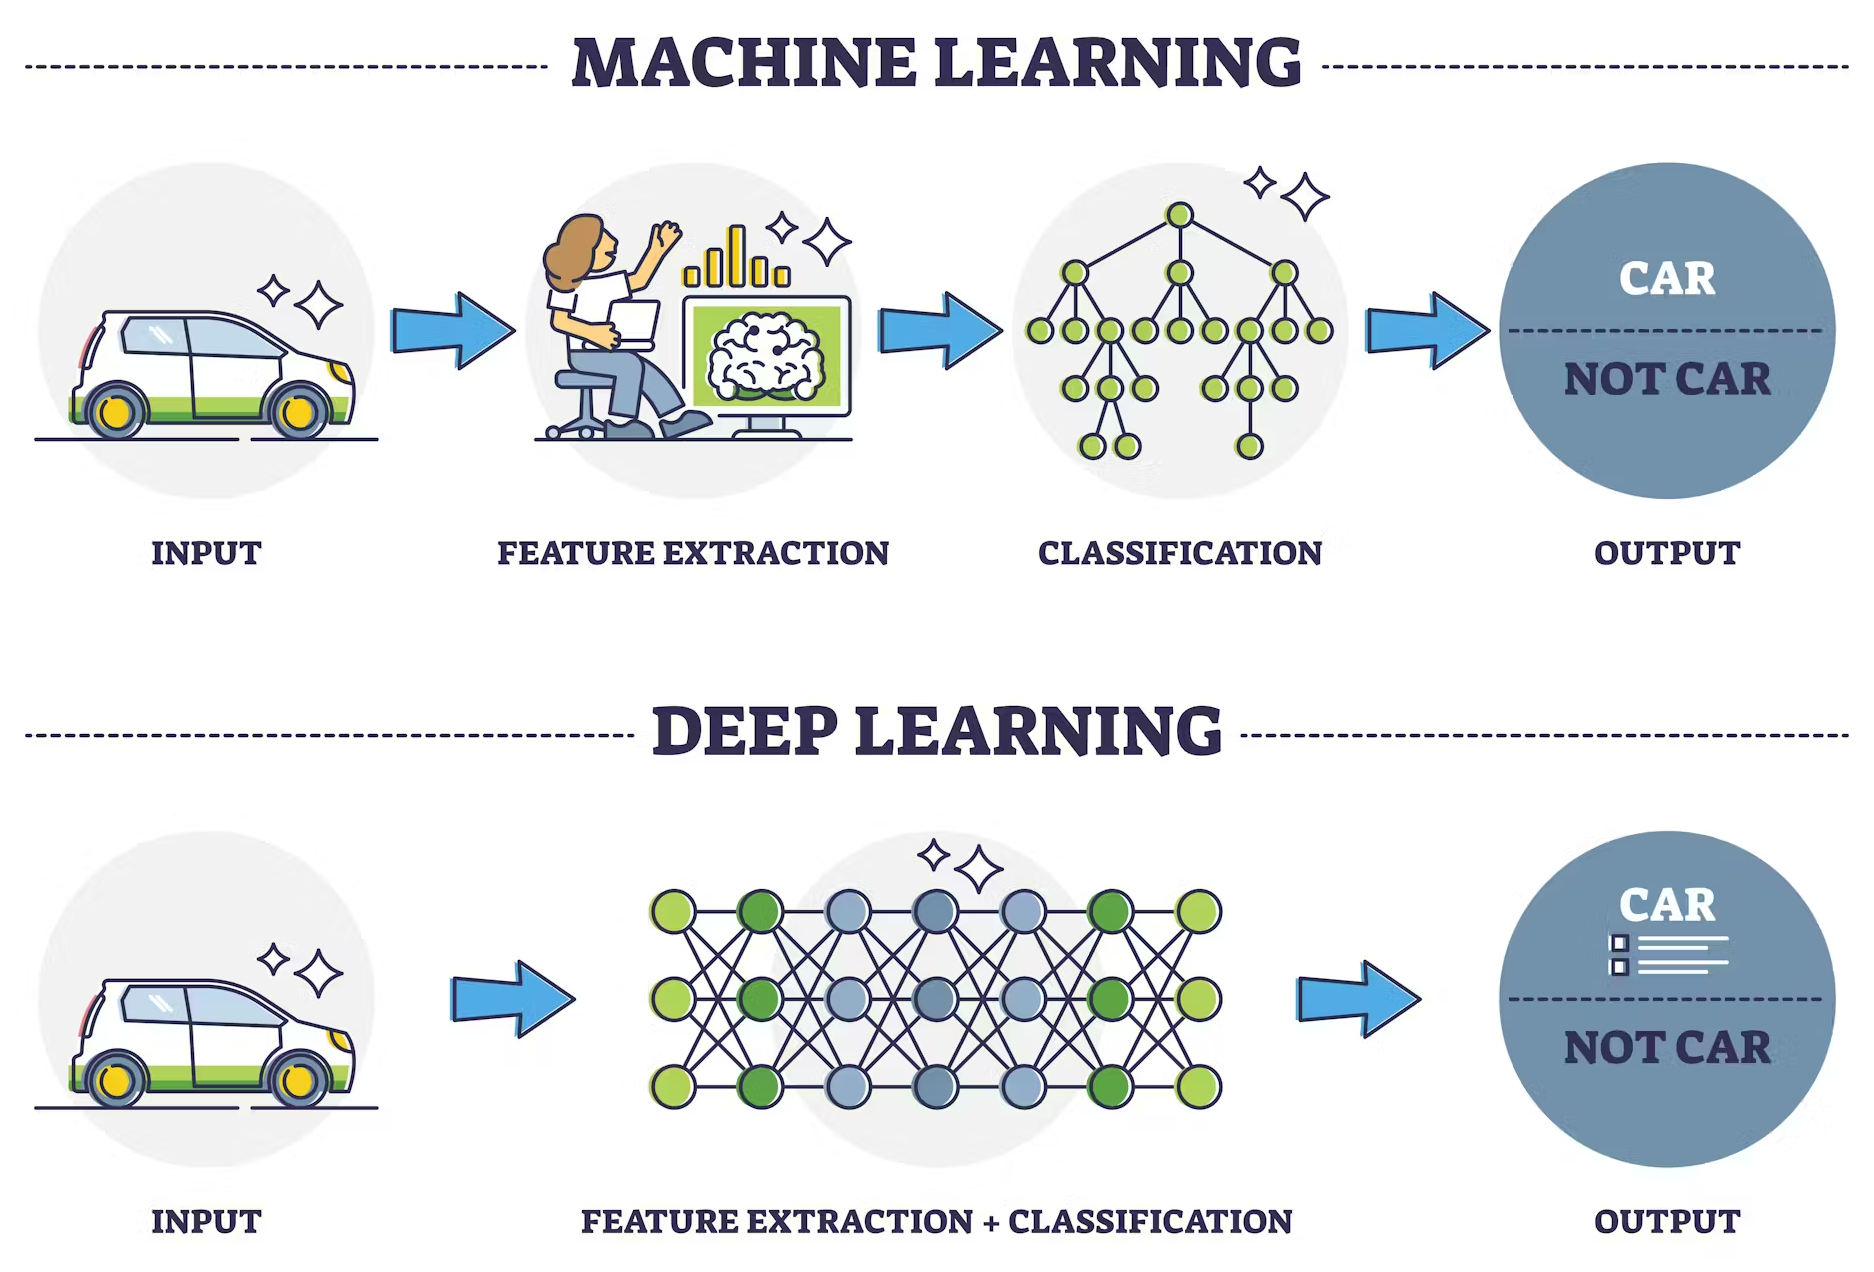
\includegraphics[scale=0.28]{images/chap2/machine_learning_vs_deep_learning.png}%
	\caption{%
بیان مفهوم پایه‌ای در تفاوت یادگیری ماشین و یادگیری عمیق
		\cite{AIT2024Deep}.
	}
	\label{machine_learning_vs_deep_learning}
	\centering
\end{figure}



یادگیری عمیق برای تنظیم وزن‌های شبکه عصبی از الگوریتم‌های بهینه‌سازی بهره می‌برد. یکی از این الگوریتم‌ها، گرادیان نزولی%
\LTRfootnote{Gradient Descent}
است که با تعیین شیب تابع هزینه%
\LTRfootnote{Loss Function}%
، وزن‌ها را به‌طور مکرر به‌روزرسانی می‌کند تا به کمترین مقدار ممکن برای این تابع برسد. الگوریتم انتشار به عقب%
\LTRfootnote{Backpropagation}
یکی از مهم‌ترین روش‌ها در این زمینه است که از گرادیان نزولی برای بهینه‌سازی وزن‌ها استفاده می‌کند. در این فرآیند، ابتدا خطای خروجی شبکه محاسبه می‌شود و سپس این خطا به‌صورت معکوس از لایه خروجی به سمت لایه‌های ورودی منتقل می‌شود تا وزن‌ها تنظیم شوند و شبکه به دقت مطلوب دست یابد.


\subsection{فرمول‌های پایه در یادگیری عمیق}
\begin{itemize}
\item تابع هزینه و انتشار به عقب

تابع هزینه یا تابع خطا معیاری است که اختلاف بین خروجی پیش‌بینی شده و مقدار واقعی را اندازه‌گیری می‌کند. یکی از توابع هزینه رایج، میانگین مربعات خطا%
\LTRfootnote{Mean Squared Error}
\lr{(MSE)}
است:
\begin{equation}
	J(\theta) = \frac{1}{m} \sum_{i=1}^{m} (y_i - \hat{y}_i)^2
\end{equation}
که در آن
$y_i$
مقدار واقعی،
$\hat{y}_i$
مقدار پیش‌بینی شده و
$m$
تعداد نمونه‌ها است. الگوریتم انتشار به عقب از این تابع هزینه استفاده می‌کند تا وزن‌ها را به‌روزرسانی کند. این فرآیند شامل محاسبه گرادیان‌ها و به‌روزرسانی وزن‌ها در جهت کاهش خطا است.


\item بهینه‌سازی با گرادیان نزولی

بهینه‌سازی با گرادیان نزولی یکی از رایج‌ترین روش‌ها برای به‌روزرسانی وزن‌های شبکه عصبی است. رابطه به‌روزرسانی وزن‌ها به صورت زیر است:
\begin{equation}
	\theta_{j} \leftarrow \theta_{j} - \alpha \frac{\partial J(\theta)}{\partial \theta_{j}}
\end{equation}
که در آن
$\theta_{j}$
وزن،
$\alpha$
نرخ یادگیری و
$\frac{\partial J(\theta)}{\partial \theta_{j}}$
مشتق جزئی تابع هزینه نسبت به وزن
$\theta_{j}$
است. این فرآیند تکرار می‌شود تا تابع هزینه به حداقل مقدار خود برسد.
\end{itemize}


\subsection{ارتباط مفاهیم یادگیری عمیق با یادگیری فدرال}
یادگیری فدرال از مفاهیم پایه‌ای یادگیری عمیق و شبکه‌های عصبی بهره می‌برد، اما از ساختاری توزیع‌شده استفاده می‌کند که در آن داده‌ها بین چندین دستگاه تقسیم شده‌اند. در یادگیری فدرال، مدل‌های یادگیری عمیق به‌صورت محلی بر روی دستگاه‌های کاربران آموزش داده می‌شوند و تنها به‌روزرسانی‌های مدل به سرور مرکزی ارسال می‌شود. این روش، علاوه بر حفظ حریم خصوصی داده‌ها، امکان استفاده از داده‌های گسترده و متنوع را فراهم می‌کند. الگوریتم‌های بهینه‌سازی مانند گرادیان نزولی و انتشار به عقب به صورت محلی اجرا شده و نتایج این به‌روزرسانی‌ها به صورت تجمیعی برای بهبود مدل کلی به کار می‌روند. این ویژگی، یادگیری فدرال را به یک رویکرد قدرتمند برای مدل‌سازی در محیط‌های توزیع‌شده تبدیل می‌کند.



\subsection{
	بیان ریاضی یادگیری فدرال
}\label{sec_FL_math}
برای بررسی مباحث ریاضی پایه در یادگیری فدرال، ابتدا باید مسئله بهینه‌سازی که در این زمینه مطرح می‌شود، به‌طور دقیق تعریف گردد. در یادگیری فدرال، هدف اصلی یافتن مجموعه‌ای از پارامترهای مدل است که عملکرد کلی مدل را بر روی داده‌های توزیع‌شده بین تعداد زیادی دستگاه بهینه کند. هر دستگاه دارای داده‌های محلی است و یک تابع هزینه محلی بر اساس این داده‌ها برای آن دستگاه تعریف می‌شود. مسئله بهینه‌سازی کلی در یادگیری فدرال به دنبال کمینه کردن مجموع وزنی این توابع هزینه محلی است تا یک مدل جامع و یکپارچه حاصل شود.

یک روش به‌روزرسانی همزمان در دوره‌های ارتباطی اجرا می‌شود. در این سیستم، یک مجموعه ثابت از
$K$
کاربر وجود دارد که هر کدام دارای یک مجموعه داده محلی ثابت هستند. در ابتدای هر دوره، یک زیرمجموعه تصادفی شامل
$C$
کاربر‌ انتخاب می‌شود و سرور وضعیت فعلی پارامترهای مدل سراسری را به هر یک از این کاربر‌ها ارسال می‌کند. هر کاربر انتخاب ‌شده سپس بر اساس وضعیت سراسری و مجموعه داده محلی خود محاسبات محلی را انجام می‌دهد و یک به‌روزرسانی به سرور ارسال می‌کند. سپس سرور این به‌روزرسانی‌ها را بر روی وضعیت سراسری خود اعمال می‌کند و این فرآیند تکرار می‌شود
\cite{mcmahan2017communication}.
تمامی رابطه‌های مورد استفاده در بخش
\ref{sec_FL_math}%
، از مرجع 
\cite{mcmahan2017communication} 
برگرفته شده‌اند.

در حالی که تمرکز بر اهداف شبکه عصبی غیرمحدب%
\LTRfootnote{non-Convex}
است، الگوریتم مورد بررسی برای هر هدف جمع-متناهی%
\LTRfootnote{Finite-Sum}
به صورت زیر قابل اعمال خواهد بود.
\begin{equation}
	\min _{w \in \mathbb{R}^d} f(w) \quad \text { where } \quad f(w) \stackrel{\text { def }}{=} \frac{1}{n} \sum_{i=1}^n f_i(w)
	\label{eq_base}
\end{equation}
برای یک مسئله یادگیری ماشین، معمولاً
$f_i(w)=\ell\left(x_i, y_i ; w\right)$
در نظر گرفته می‌شود، به این معنی که این تابع نشان‌دهنده‌ی خطای پیش‌بینی بر روی نمونه
$(x_i, y_i)$
با استفاده از پارامترهای مدل
$w$
است. فرض می‌شود که داده‌ها بین
$K$
کاربر تقسیم شده‌اند، که در آن
$\mathcal{P}_k$
مجموعه‌ای از نقاط داده مربوط به کاربر
$k$
است و
$n_k=\left|\mathcal{P}_k\right|$
تعداد این نقاط داده را نشان می‌دهد. بنابراین، با توجه به این مورد می‌توان رابطه
\eqref{eq_base}
را به صورت زیر بازنویسی نمود:
\begin{equation}
	f(w)=\sum_{k=1}^K \frac{n_k}{n} F_k(w) \quad \text { where } \quad F_k(w)=\frac{1}{n_k} \sum_{i \in \mathcal{P}_k} f_i(w)
\end{equation}

%اگر مجموعه
%$\mathcal{P}_k$
%با توزیع یکنواخت%
%\LTRfootnote{Uniform Distribution}
%تصادفی از مثال‌های آموزشی بین کاربر‌ها تشکیل شده باشد، در آن صورت
%$\mathbb{E}_{\mathcal{P}_k}\left[F_k(w)\right]=f(w)$ 
%خواهد بود، که در این جا امید ریاضی بر روی مجموعه مثال‌های اختصاص داده شده به یک کاربر ثابت گرفته می‌شود.
اگر مجموعه 
$\mathcal{P}_k$ 
به صورت تصادفی و با توزیع یکنواخت%
\LTRfootnote{Uniform Distribution}
از نمونه‌های آموزشی بین کاربر‌ها تشکیل شده باشد، در این صورت 
$\mathbb{E}_{\mathcal{P}_k}\left[F_k(w)\right]$ 
برابر
$f(w)$ 
خواهد بود. به این معنا که امید ریاضی بر روی مجموعه مثال‌های اختصاص داده شده به یک کاربر خاص، محاسبه می‌شود.
این همان فرض
استقلال و توزیع یکنواخت داده‌ها%
\LTRfootnote{Independent and Identically Distributed}
\lr{(IID)}
است که عموماً توسط الگوریتم‌های بهینه‌سازی توزیع‌شده استفاده می‌شود. در این‌جا حالتی که فرض مذکور برقرار نیست (یعنی
$F_k$
می‌تواند تقریباً به هر میزانی از
$f$
فاصله داشته باشد)، به عنوان حالت
غیرمستقل و غیریکنواخت
\lr{(non-IID)}
شناخته می‌شود
\cite{mcmahan2017communication}.
جهت درک بهتر به شکل
\ref{iid_vs_noniid}
توجه نمایید.


\begin{figure}[t]
	\centering
	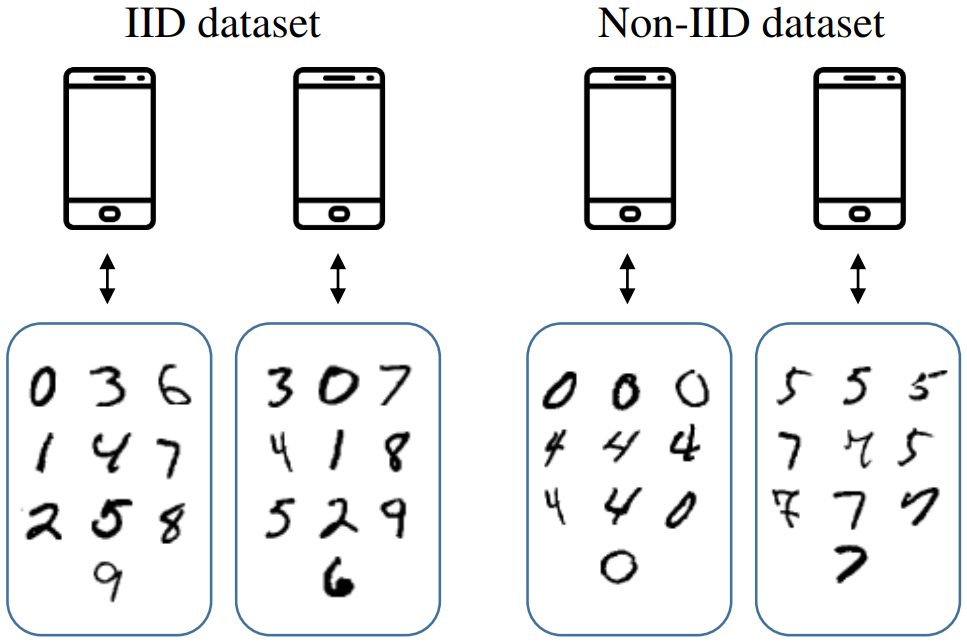
\includegraphics[scale=0.4]{images/chap2/iid_vs_noniid.png}%
	\caption{%
		تفاوت ساختار
		\lr{IID}
		با
		\lr{non-IID}
		\cite{hellström2022wirelessmachinelearning}.
	}
	\label{iid_vs_noniid}
	\centering
\end{figure}



\section{چالش‌های موجود در یادگیری فدرال و نگاه کلی مقالات به آن‌ها}
با وجود اینکه یادگیری فدرال نسبت به روش‌های سنتی یادگیری ماشین دارای مزایای قابل توجهی است، اما به دلیل ساختار شبکه‌ای خود با چالش‌های متعددی روبرو است. در ادامه، مهم‌ترین چالش‌های یادگیری فدرال مورد بررسی قرار گرفته و به دیدگاه‌های کلی مقالات علمی در مورد این چالش‌ها اشاره می‌شود.


\subsection{چالش تبادل داده}
تبادل داده بین سرور و کاربران به دلیل مشکلات پهنای باند و ارتباطات شبکه‌ای اصولا کار پر هزینه‌ای می‌باشد. یکی از دلایل اصلی پرهزینه بودن این ارتباطات، حجم بالای داده‌هایی است که باید بین دستگاه‌های کاربری و سرور منتقل شوند.
معمولاً مشکلات ارتباطی به انتقال‌های بسیار زیاد به‌روزرسانی‌های مدل بین گره‌های محاسباتی نسبت داده می‌شود. با افزایش تعداد پارامترها در مدل‌های پیشرفته، اندازه این مدل‌ها نیز به طور متناسب بزرگ می‌شود
\cite{wang2018atomo}.

از سوی دیگر، مشارکت تعداد زیادی از دستگاه‌های کاربران نهایی در فرآیند آموزش مدل‌ها، می‌تواند هزینه‌های ارتباطی را به طور قابل توجهی افزایش دهد. همچنین، به علت مشکلات ارتباطی، در بسیاری از مواقع تمامی دستگاه‌ها در هر چرخه از فرآیند آموزش حضور ندارند. این موضوع باعث افزایش هزینه‌ها و پیچیدگی‌های مرتبط با انتقال داده‌ها می‌شود، زیرا زمانی که تنها بخشی از دستگاه‌ها در فرآیند آموزش شرکت می‌کنند، هماهنگی، انتخاب کاربران و تجمیع نتایج از این دستگاه‌ها نیازمند مدیریت پیچیده‌تری است که منجر به افزایش هزینه‌های کلی می‌شود.


استفاده از فشرده‌سازی داده‌ها می‌تواند هزینه‌های ارتباطی را به میزان قابل توجهی کاهش دهد. برای مدیریت هزینه‌های بالای ارتباطات در فرآیند یادگیری فدرال، روش‌هایی مورد بررسی قرار گرفته‌اند که بر فشرده‌سازی داده‌های ارسالی از دستگاه‌های نهایی به سرور مرکزی تمرکز دارند. این تکنیک‌ها با کاهش حجم اطلاعات ارسالی، به کاهش هزینه‌های ارتباطی کمک می‌کنند
\cite{konevcny2016federated}.

در این راستا روشی به نام
\lr{PCFL}%
\LTRfootnote{Privacy Communication efficient Federated Learning}
در
\cite{fang2021privacy}
ارائه شده است که از نظر ارتباطی بسیار کارآمد بوده و شامل سه عنصر اصلی می‌باشد. این عناصر شامل فشرده‌سازی دوطرفه، فشرده‌سازی مکانی وزن‌ها و یک پروتکل پیشرفته برای حفظ حریم خصوصی داده‌ها هستند. فشرده‌سازی دوطرفه، داده‌ها را در دو مرحله، هم قبل از ارسال از دستگاه‌های نهایی به سرور و هم هنگام ارسال نتایج به‌روزرسانی‌شده از سرور به دستگاه‌ها، فشرده می‌کند تا حجم داده‌های انتقالی کاهش یابد. فشرده‌سازی مکانی وزن‌ها نیز با فشرده کردن وزن‌های مدل، حجم انتقال را کاهش داده و کارایی ارتباطات را بهبود می‌بخشد. پروتکل حفظ حریم خصوصی داده‌ها نیز امنیت اطلاعات کاربران را در طول فرآیند یادگیری فدرال تضمین می‌کند. این عناصر با همکاری هم، موجب کاهش هزینه‌های ارتباطی و بهبود کارایی در روش
\lr{PCFL}
می‌شوند.



\subsection{
	چالش ناهمگنی‌های سیستمی%
\LTRfootnote{Systems Heterogeneity}
}
در دنیای یادگیری فدرال، دستگاه‌ها از نظر حافظه، توان محاسباتی و ارتباطات بسیار با یکدیگر متفاوت هستند. این تفاوت‌ها ممکن است از اختلافاتی مانند تفاوت در پردازنده، نوع حافظه، نوع اتصال شبکه و نیاز به انرژی ناشی شود. علاوه بر این محدودیت‌های موجود در شبکه و سیستمی می‌توانند باعث ایجاد وضعیت‌هایی شوند که برخی از دستگاه‌ها در یک زمان معین در دسترس نباشند. برای مثال، اگر تعداد زیادی دستگاه به صورت همزمان درخواست ارسال داشته باشند، ممکن است برخی از آن‌ها به دلیل پهنای باند محدود یا محدودیت‌های سخت‌افزاری، قادر به ارسال درخواست نشوند. همچنین، ممکن است یک دستگاه فعال، به دلیل مشکلاتی مانند اختلالات در شبکه یا مصرف اضافی انرژی، از فرآیند یادگیری خارج شود.

این تفاوت‌های سیستمی، یکی از چالش‌های یادگیری فدرال محسوب می‌شوند و می‌توانند باعث افزایش تأخیر و ایجاد اشکالات در سیستم شوند. بنابراین، برای رفع این مشکلات، روش‌های یادگیری فدرال باید توانایی پیش‌بینی دقیق تعداد دستگاه‌هایی که در هر فرآیند شرکت می‌کنند را داشته باشند. همچنین، باید بتوانند در برابر دستگاه‌هایی که در حین عملیات دچار مشکل شده و از دسترس خارج می‌شوند، مقاومتی مناسب داشته باشند
\cite{li2020federated}.


برای مقابله با ناهمگنی سیستمی، روشی تحت عنوان تعادل در به‌روزرسانی مدل مطرح شده است
\cite{konevcny2015federated}.
در این روش، وزن‌دهی به نمونه‌ها بر اساس میزان نیاز به آموزش در هر دستگاه صورت می‌گیرد. این کار باعث می‌شود که دستگاه‌های با حجم داده کمتر، وزن بیشتری در به‌روزرسانی مدل داشته باشند.
در رویکرد دیگری به نام یادگیری فعال، دستگاه‌هایی که داده‌های خود را به سرور ارسال می‌کنند، فعالیت خود را به نحوی تنظیم می‌کنند که مدل از داده‌های مهم‌تر و کمتر دیده شده بیشتر یاد می‌گیرد
\cite{konevcny2016federated}.
این روش می‌تواند به تعادل در آموزش مدل کمک کند و از ناهمگنی سیستمی جلوگیری کند.


\subsection{
	چالش ناهمگنی‌های آماری%
\LTRfootnote{Statistical Heterogeneity}
}
روش‌های مختلفی برای تولید و جمع‌آوری داده‌ها بین دستگاه‌ها وجود دارد. این داده‌ها معمولاً به صورت مستقل از هم تولید نمی‌شوند و بین آن‌ها ارتباطات و پیوندهایی وجود دارد. چنین الگویی از تولید داده با فرضیات استقلال و توزیع یکنواخت داده‌ها
\lr{(IID)}
در مسائل بهینه‌سازی در تضاد است، که منجر به پیچیدگی‌هایی در فرآیند مدل‌سازی، تحلیل نظری و ارزیابی عملکرد می‌شود. بنابراین، با وجود هدف نهایی که یادگیری یک مدل جامع و یکپارچه است، روش‌های جایگزین مانند یادگیری چندوظیفه‌ای%
\LTRfootnote{Multi-Tasking}
و فرایادگیری%
\LTRfootnote{Meta Learning}
به عنوان راه‌حل‌های ممکن مطرح شده‌اند
\cite{li2020federated}.


یک روش برای حل مشکل ناهمگنی آماری در یادگیری فدرال استفاده از رویکرد ترکیبی یا ترکیب روش‌های یادگیری محلی است
\cite{konevcny2015federated}.
در این رویکرد، به جای استفاده از یک الگوریتم یادگیری مشترک برای تمام دستگاه‌ها، از چندین الگوریتم یادگیری محلی با تنوع مدل‌ها و تنظیمات مختلف استفاده می‌شود. سپس، اطلاعات مدل‌های محلی روی سرور یا گره مرکزی جمع‌آوری می‌شود و با استفاده از ترکیب این اطلاعات، یک مدل یادگیری مشترک به‌روزرسانی خواهد شد.



\subsection{چالش حریم شخصی}\label{privacy_challenge}
حفظ حریم شخصی یک مزیت مهم در یادگیری فدرال به شمار می‌رود، اما در صورت عدم کنترل مناسب می‌تواند به یک چالش تبدیل شود. یکی از چالش‌های اساسی در این زمینه، محافظت از حریم شخصی کاربران است که به دلیل قرار گرفتن داده‌های حساس در اختیار بخش‌های مختلف شبکه، اهمیت بیشتری پیدا می‌کند.

اگرچه در یادگیری فدرال، تنها مدل‌های به‌روز شده یا گرادیان‌های آن‌ها به سرور مرکزی ارسال می‌شوند و داده‌های خام کاربران هرگز از دستگاه‌های محلی خارج نمی‌شوند. به عبارتی، تنها وزن‌های شبکه‌های عصبی که حاوی اطلاعات مستقیم شناسایی فردی نیستند، مبادله می‌شوند. با این وجود، همچنان چالش‌هایی در حفظ حریم شخصی وجود دارد. 

مدل‌های به‌روزرسانی‌ شده ممکن است به صورت غیرمستقیم حاوی الگوهایی از داده‌های حساس باشند که در فرآیند آموزش استفاده شده‌اند. این الگوها می‌توانند توسط مهاجمان تحلیل شده و اطلاعاتی در مورد داده‌های کاربران را افشا کنند. برای مثال، حملات بازسازی داده یا حملات استنتاج می‌توانند با دسترسی به وزن‌های به‌روزرسانی شده، داده‌های اولیه را تا حدی بازسازی کنند. بنابراین، حتی اگر داده‌های خام مستقیماً ارسال نشوند، نیاز به تدابیر امنیتی برای جلوگیری از این نوع حملات وجود دارد. در نتیجه، اگرچه یادگیری فدرال حریم شخصی را بهتر حفظ می‌کند، اما همچنان نیازمند روش‌های پیشرفته امنیتی مانند رمزنگاری، تنظیم نویز در داده‌ها و روش‌های دیگر برای تضمین حفاظت از حریم شخصی کاربران است.


روش حفظ حریم خصوصی تفاضلی%
\LTRfootnote{Differential Privacy}
با افزودن نویز به نتایج محاسبات یا به داده‌های ورودی، اطمینان حاصل می‌کند که حضور یا عدم حضور یک نمونه داده خاص در مجموعه داده‌ها، تأثیر قابل توجهی بر خروجی محاسبات نداشته باشد. این روش به ویژه برای حفظ حریم خصوصی در یادگیری فدرال مفید است زیرا از افشای اطلاعات حساس از طریق پارامترهای مدل جلوگیری می‌کند
\cite{hasan2023security}.

یک روش دیگر، رویکرد رمزنگاری هم‌شکل%
\LTRfootnote{Homomorphic Encryption}
است که امکان محاسبه روی داده‌های رمزنگاری شده را بدون نیاز به رمزگشایی آن‌ها فراهم می‌کند. این رویکرد به ویژه در یادگیری فدرال برای حفظ حریم خصوصی داده‌ها در حین انجام محاسبات مفید است زیرا نیاز به تغییر ماهیت داده نبوده و چون جابه‌جایی در یادگیری فدرال زیاد رخ می‌دهد، این رویکرد بسیار کارا خواهد بود
\cite{yin2021comprehensive}.



\section{رویکردهای کلی و پایه‌ای در حل چالش‌ها}
روش‌های بهینه‌سازی توزیع‌شده معمولاً برای حل مسائل بهینه‌سازی در سیستم‌هایی با شبکه‌های محاسباتی بزرگ و توزیع‌شده استفاده می‌شوند. این روش‌ها بر مبنای تقسیم مسئله بهینه‌سازی به زیرمسائل کوچک‌تر و حل آن‌ها در گره‌های مختلف شبکه استوارند. در این روش‌ها، اغلب فرض می‌شود که داده‌ها به صورت همگن و یکپارچه در سراسر شبکه توزیع شده‌اند و گره‌ها می‌توانند به راحتی با یکدیگر ارتباط برقرار کنند.

این فرضیات در یادگیری فدرال به ندرت برقرار است، زیرا در یادگیری فدرال داده‌ها به صورت محلی و ناهمگن در دستگاه‌های مختلف قرار دارند و ارتباطات بین دستگاه‌ها ممکن است محدود و نامنظم باشد
\cite{konevcny2015federated}.
بنابراین روش‌ها و رویکردهای لازم جهت حل این چالش‌ها متفاوت از مسائل بهینه‌سازی توزیع شده هستند. در این مرحله، تلاش می‌شود دو رویکرد پایه‌ای برای مسائل یادگیری فدرال معرفی شود.


\subsection{
	الگوریتم میانگین‌گیری فدرال%
	\LTRfootnote{Federated Averaging}
	\lr{\texttt{\fontspec{Times New Roman} (FedAvg)}}
}
یکی از روش‌های اصلی و پرکاربرد در یادگیری فدرال روش میانگین‌گیری فدرال یا
\lr{FedAvg}
است که توسط محققان گوگل در سال 2017 معرفی شد
\cite{mcmahan2017communication}.
این الگوریتم به منظور بهینه‌سازی مدل‌های یادگیری ماشین در یک محیط توزیع‌شده طراحی شده است. در این روش داده‌ها به صورت محلی در دستگاه‌های کاربران باقی می‌مانند و تنها به‌روزرسانی‌های مدل به اشتراک گذاشته می‌شوند. رویکرد اصلی
\lr{FedAvg}
بر مبنای ترکیب به‌روزرسانی‌های محلی از دستگاه‌های مختلف به یک مدل سراسری استوار است.


یکی از مزایای اصلی
\lr{FedAvg}
این است که به طور موثری با چالش ناهمگنی داده‌ها مقابله می‌کند. در یادگیری فدرال، داده‌های موجود در دستگاه‌های مختلف ممکن است توزیع‌های متفاوتی داشته باشند. این ناهمگنی می‌تواند به دلیل تفاوت در رفتار کاربران یا حتی محیط‌های مختلف جمع‌آوری داده باشد. میانگین‌گیری وزنی در
\lr{FedAvg}
به مدل کمک می‌کند تا به‌روزرسانی‌های مختلف را به گونه‌ای ترکیب کند که این ناهمگنی‌ها را در نظر بگیرد. به عبارت دیگر، اگر یک دستگاه داده‌های بیشتری داشته باشد، تأثیر بیشتری بر مدل نهایی خواهد داشت. این رویکرد باعث می‌شود که مدل فدرال به تعادل بهتری در یادگیری از داده‌های ناهمگن برسد و کارایی بالاتری داشته باشد. این ویژگی به ویژه در کاربردهایی مانند فروشگاه برنامه‌های کاربردی که کاربران متنوع و داده‌های متفاوتی دارند، بسیار سودمند است و می‌تواند به بهبود عملکرد مدل در شرایط واقعی کمک شایانی کند.

علاوه بر این،
\lr{FedAvg}
به کاهش نیاز به ارتباطات مکرر بین دستگاه‌ها و سرور مرکزی کمک می‌کند. در بسیاری از روش‌های بهینه‌سازی توزیع‌شده، نیاز است که دستگاه‌ها به طور مکرر با سرور مرکزی ارتباط برقرار کنند تا به‌روزرسانی‌های خود را ارسال کنند. اما در
\lr{FedAvg}
دستگاه‌ها می‌توانند چندین مرحله از بهینه‌سازی را به صورت محلی انجام دهند و سپس تنها به‌روزرسانی نهایی را ارسال کنند. این کاهش در نیاز به ارتباطات نه تنها باعث کاهش پهنای باند مورد نیاز می‌شود، بلکه به حفظ حریم خصوصی کاربران نیز کمک می‌کند، زیرا داده‌ها هرگز از دستگاه‌های محلی خارج نمی‌شوند. بررسی‌ها نشان داده‌اند که متناسب با اندازه داده‌ها، پس از رسیدن به تعداد مشخصی از گره، اضافه کردن گره‌های بیشتر، تأثیری در کاهش هزینه‌های ارتباطی نخواهد داشت. در چنین شرایطی، تمرکز بر افزایش توان محاسباتی محلی یا تعداد مراحل آموزش محلی می‌تواند موجب تسریع فرایند آموزش شود
\cite{mcmahan2017communication}.

برای درک چگونگی پیدایش الگوریتم
\lr{FedAvg}%
، باید به این نکته اشاره کرد که موفقیت‌های اخیر در یادگیری عمیق عمدتاً به استفاده از انواع الگوریتم نزول گرادیان تصادفی%
\LTRfootnote{Stochastic Gradient Descent}
\lr{(SGD)}
برای بهینه‌سازی وابسته بوده‌اند. در حقیقت، بسیاری از دستاوردها، ناشی از تنظیم مدل و بهینه‌سازی تابع خطا با استفاده از روش‌های ساده گرادیان هستند. از این رو، منطقی است که الگوریتم‌های بهینه‌سازی فدرال نیز با الگوریتم
\lr{SGD}
به عنوان نقطه شروع، طراحی و توسعه یابند
\cite{mcmahan2017communication}.

%موفقیت‌های اخیر در کاربردهای یادگیری عمیق تقریباً به‌طور انحصاری به استفاده از انواع الگوریتم نزول گرادیان تصادفی%
%\LTRfootnote{Stochastic Gradient Descent}
%\lr{(SGD)}
%برای بهینه‌سازی متکی بوده‌اند. در واقع، بسیاری از پیشرفت‌ها به تنظیم مدل و بهینه‌سازی تابع خطا با روش‌های ساده گرادیان مربوط می‌شود. بنابراین، منطقی است که الگوریتم‌های بهینه‌سازی فدرال با شروع از
%\lr{SGD}
%طراحی و توسعه یابند
%\cite{mcmahan2017communication}.

الگوریتم
\lr{SGD}
می‌تواند به سادگی در بهینه‌سازی فدرال استفاده شود، به این صورت که در هر دور ارتباط، گرادیان‌ها بر اساس داده‌های یک کاربر تصادفی انتخاب شده، محاسبه ‌شوند. این رویکرد از نظر محاسباتی کارآمد است، اما نیازمند تعداد بسیار زیادی از دورهای آموزش برای تولید مدل‌های مناسب است.
برای مثال حتی با استفاده از رویکرد پیشرفته‌ای مانند نرمال‌سازی دسته‌ای%
\LTRfootnote{Batch Normalization}%
، برای آموزش مجموعه‌داده‌ای تنها با 60٬000 داده ورودی و
با دسته‌های کوچکی به اندازه 60، به 50٬000 دور آموزش جهت رسیدن به مدل مطلوب نیاز می‌باشد
\cite{ioffe2015batch}.

در تنظیمات فدرال، مشارکت تعداد زیادی از کاربران هزینه چندانی در زمان واقعی ندارد زیرا همه کاربران می‌توانند به صورت همزمان به آموزش مدل محلی بپردازند. بنابراین، برای خط مبنا از
\lr{SGD}
همزمان با دسته‌های بزرگ استفاده می‌شود. برای اعمال این رویکرد در تنظیمات فدرال، در هر دور یک زیرمجموعه‌ای از کاربران با ضریب کنترلی 
$C$
انتخاب می‌شوند و گرادیان خطا روی تمام داده‌های نگهداری شده توسط این کاربران محاسبه می‌گردد. بنابراین،
$C$
اندازه دسته کلی را کنترل می‌کند، به‌طوری که
$C = 1$
معادل با نزول گرادیان یک دسته کامل است. این الگوریتم خط مبنا
\lr{FederatedSGD}
یا
\lr{FedSGD}
نامیده می‌شود
\cite{mcmahan2017communication}.


یک پیاده‌سازی معمول از
\lr{FedSGD}
با
$C = 1$
و نرخ یادگیری ثابت
$\eta$
به این صورت است که هر گره
$k$%
، گرادیان
$g_k=\nabla F_k\left(w_t\right)$
که میانگین گرادیان روی داده‌های محلی در مدل فعلی
$w_t$
است را محاسبه می‌کند و سرور مرکزی این گرادیان‌ها را جمع‌آوری کرده و به‌روزرسانی
$w_{t+1} \leftarrow w_t-\eta \sum_{k=1}^K \frac{n_k}{n} g_k$
را انجام می‌دهد، در حالی که
$\sum_{k=1}^K \frac{n_k}{n} g_k=\nabla f\left(w_t\right)$
خواهد بود. یک به‌روزرسانی معادل به این صورت است که برای هر گره عبارت
$\forall k, w_{t+1}^k \leftarrow w_t-\eta g_k$
محاسبه و سپس
$w_{t+1} \leftarrow \sum_{k=1}^K \frac{n_k}{n} w_{t+1}^k$
انجام شود.

در نتیجه، هر گره به صورت محلی یک گام گرادیان نزولی را روی مدل فعلی با استفاده از داده‌های محلی خود انجام داده و سپس سرور میانگین وزنی مدل‌های به‌دست‌آمده را محاسبه می‌کند. با نوشتن الگوریتم به این صورت، امکان تکرار به‌روزرسانی محلی
$w^k \leftarrow w^k-\eta \nabla F_k\left(w^k\right)$%
، چندین بار پیش از مرحله میانگین‌گیری فراهم شده و باعث افزایش محاسبات در هر گره خواهد شد. الگوریتم
\lr{FederatedAveraging}
یا
\lr{FedAvg}
به این صورت به وجود آمد
\cite{mcmahan2017communication}.
جهت درک بهتر این ساختار، می‌توان شکل 
\ref{federated_learning} 
را مشاهده نمود و در گام سوم به میانگین وزنی مدل‌ها توجه کرد.

در این روش میزان محاسبات توسط سه پارامتر کلیدی کنترل می‌شود:
\begin{itemize}
	\itemsep-1mm 
	\item
	$C$%
: زیرمجموعه‌ای از تعداد گره‌هایی که در هر مرحله محاسبات انجام می‌دهند

	\item
	$E$%
: تعداد مراحل آموزشی که هر گره در هر دور روی مجموعه داده محلی خود انجام می‌دهد
	
	\item
	$B$%
: اندازه دسته محلی که برای به‌روزرسانی‌های هر گره استفاده می‌شود
	
\end{itemize}
در این‌جا
$B = \infty$
انتخاب می‌شود تا نشان دهد که کل مجموعه داده محلی به عنوان یک دسته واحد در نظر گرفته می‌شود. بنابراین، به عنوان یک نمونه از این الگوریتم گسترده شده جدید، انتخاب
$B = \infty$
و
$E = 1$
باعث می‌شود که این روش دقیقا مانند
\lr{FedSGD}
عمل کند. همچنین برای یک گره با
$n_k$
نمونه محلی، تعداد به‌روزرسانی‌های محلی در هر دور با
$u_k=E \frac{n_k}{B}$
نمایش داده می‌شود
\cite{mcmahan2017communication}.
شبه کد کامل این روش در الگوریتم
\ref{algo_FedAvg}
ارائه شده است. علاوه بر این، تمامی نمادهای مورد استفاده در این الگوریتم در جدول
\ref{tabel_FedAvgNotations}
توضیح داده شده است. هدف از این جدول، فراهم کردن درکی جامع از نحوه عملکرد و پیاده‌سازی الگوریتم می‌باشد.


\begin{LTR}
\SetAlgoNlRelativeSize{-1}
\begin{algorithm}[t]
	\begin{RTL}
		\caption{%
میانگین‌گیری فدرال
			\lr{(FedAvg)}
			\cite{mcmahan2017communication}
		}
		\label{algo_FedAvg}
	\end{RTL}
	
	\begin{latin}
		initialize $w_0$\;
		\For{each round $t = 1, 2, \ldots, T$}{
			$m \gets \max(C \cdot K, 1)$\;
			$U_t \gets$ (random set of $m$ clients)\;
			\For{each client $k \in U_t$
				\textbf{in parallel}}{
				$w_{t+1}^k \gets \texttt{ClientUpdate}(k, w_t)$\;
			}
			$w_{t+1} \leftarrow \sum_{k=1}^K \frac{n_k}{n} w_{t+1}^k$\;
		}
		\SetKwFunction{ClientUpdate}{ClientUpdate}
		\SetKwProg{Fn}{Function}{:
		\quad // {\mdseries \textit{Run on client} $k$}
		}{end}
		\Fn{\ClientUpdate{$k, w$}}{
			$\mathcal{B} \leftarrow$ (split $\mathcal{P}_k$ into batches of size $B$)\;
			\For{each local epoch \space $i$ \space from $1$ to $E$}{
				\For{batch $b \in \mathcal{B}$}{
					$w \gets w - \eta \nabla \ell(w$%
					\texttt{\char`\~}%
					$b)$\;
				}
			}
			\KwRet $w$ to server\;
		}
	\end{latin}
\end{algorithm}
\end{LTR}


\begin{table}[h]
	\centering
	\caption{نمادهای به‌کار رفته در الگوریتم
		\lr{FedAvg}
	}
	\label{tabel_FedAvgNotations}
	\begin{tabular}{cr}
		\hline
		متغیر & توضیحات \\
		\hline
		$w$ & وزن‌های شبکه عصبی \\
		$T$ & تعداد گام‌ها \\
		$K$ & تعداد کاربران \\
		$C$ & ضریب کنترلی برای زیرمجموعه‌ای از کاربران \\
		$m$ & زیر مجموعه‌ای از کاربران \\
		$U_t$ & مجموعه‌ای نامرتب از $m$ در گام $t$ \\
		$n$ & تعداد داده‌های آموزشی \\
		$\mathcal{P}_k$ & مجموعه داده‌های متعلق به کاربر $k$ \\
		$B$ & اندازه دسته محلی \\
		$E$ & تعداد مراحل آموزش محلی \\
		$\eta$ & نرخ یادگیری
	\end{tabular}
\end{table}


\subsection{
بهینه‌سازی
\lr{\texttt{\fontspec{Times New Roman} FedProx}}
}\label{sec_FedProx}
روش
\lr{FedProx}
به بررسی چالش‌های یادگیری فدرال در بسترهای ناهمگن می‌پردازد. این روش با ایجاد تغییرات جزئی در رویکرد
\lr{FedAvg}%
، به بهبود پایداری و دقت در شبکه‌های ناهمگن کمک می‌کند. این تغییرات شامل اضافه کردن یک عبارت نزدیک‌سازی%
\LTRfootnote{Proximal Term}
به تابع هدف است که به سرور کمک می‌کند تا ناهمگنی را مدیریت کند
\cite{li2020federatedheteroneneous}.
عبارت نزدیک‌سازی، یک معنای اصطلاحی در زمینه بهینه‌سازی است که به تابعی افزوده می‌شود تا مشکلات ناشی از تفاوت‌های میان مدل‌های محلی و مدل سراسری در یادگیری فدرال را بر طرف کند.
تمامی رابطه‌های مورد استفاده در بخش
\ref{sec_FedProx}%
، از مرجع 
\cite{li2020federatedheteroneneous} 
برگرفته شده‌اند.

رابطه هدف
\lr{FedProx}
به صورت زیر تعریف می‌شود:
\begin{equation}
\min_{w} f(w) = \min_{w} \sum_{k=1}^{K} \frac{n_k}{n} \left( F_k(w) + \frac{\mu}{2} \|w_t - w_t^k\|^2 \right)
\label{eq_FedProx}
\end{equation}

در رابطه
\eqref{eq_FedProx}
بخش
$\frac{\mu}{2} \|w_t - w_t^k\|^2$%
، همان عبارت نزدیک‌سازی است که به تابع هدف اضافه شده است. همچنین
$\mu$%
، یک پارامتر تنظیم برای این عبارت به حساب می‌آید و در نهایت
$w_t^k$
وزن‌های مدل محلی دستگاه
$k$
در تکرار
$t$
است.

حال با توجه به رابطه
\eqref{eq_FedProx}%
، به‌روزرسانی وزن‌ها به شکل زیر تغییر پیدا خواهد کرد و بخش
$\mu (w_t - w_t^k)$%
، گرادیان عبارت نزدیک‌‌سازی است.
\begin{equation}
w_{t+1} = w_t - \eta (\nabla F_k(w_t) + \mu (w_t - w_t^k))
\end{equation}

بنابراین، به‌روزرسانی‌های محلی در هر گام با به‌روزرسانی سراسری مرحله قبل مرتبط هستند. در حقیقت عبارت نزدیک‌سازی به عنوان یک مکانیزم منظم‌کننده%
\LTRfootnote{Regularization}
عمل می‌کند که تفاوت‌های بین وزن‌های سراسری
$w$
و وزن‌های محلی
$w_t^k$
را کاهش می‌دهد. این عبارت به کاهش تاثیرات منفی ناهمگنی سیستم‌ها و داده‌ها کمک می‌کند و باعث پایداری بیشتر در فرآیند همگرایی می‌شود
\cite{li2020federatedheteroneneous}.


\section{جمع‌بندی}
یادگیری فدرال به عنوان یک چارچوب نوین در یادگیری ماشین، از مفاهیم پایه یادگیری ماشین و یادگیری عمیق بهره می‌برد، اما با ساختاری توزیع‌شده که در آن داده‌ها بین چندین دستگاه پخش می‌شود. در فرایند یادگیری فدرال، الگوریتم‌های بهینه‌سازی مانند گرادیان نزولی و انتشار به عقب به‌طور محلی اجرا می‌شوند و سپس نتایج این به‌روزرسانی‌ها با هم ترکیب می‌شوند تا مدل کلی بهبود یابد.

یادگیری فدرال با چالش‌هایی چون تبادل داده‌های پرهزینه، ناهمگنی‌های سیستمی و آماری، و حفظ حریم شخصی مواجه است. به دلیل حجم بالای داده‌ها، تبادل اطلاعات بین سرور و دستگاه‌ها پرهزینه است و روش‌هایی مانند فشرده‌سازی داده‌ها برای کاهش این هزینه‌ها پیشنهاد شده است. همچنین، ناهمگنی در توان محاسباتی و آماری دستگاه‌ها می‌تواند تأثیرات منفی بر فرایند یادگیری داشته باشد که با روش‌هایی مانند تعادل در به‌روزرسانی مدل‌ها و یادگیری فعال می‌توان این مشکلات را به حداقل رساند. حفظ حریم خصوصی نیز چالشی جدی است و برای مقابله با آن روش‌های امنیتی پیشرفته‌ای نظیر حریم خصوصی تفاضلی و رمزنگاری هم‌شکل به کار گرفته می‌شوند.

الگوریتم‌های
\lr{FedAvg}
و
\lr{FedProx}
به عنوان رویکردهای پایه‌ای در یادگیری فدرال، چالش‌های مرتبط با ناهمگنی داده‌ها و تفاوت‌های سیستمی را هدف قرار می‌دهند.
\lr{FedAvg}
با جمع‌آوری و میانگین‌گیری وزن‌های مدل‌های محلی که توسط کاربران آموزش دیده‌اند، به یک مدل سراسری همگرا می‌شود، اما در برابر تنوع داده‌ها و دستگاه‌ها حساس است.
\lr{FedProx}
با اضافه کردن یک عبارت جریمه به تابع هدف، سعی می‌کند ناهماهنگی بین مدل‌های محلی و مدل مرکزی را کاهش دهد و در نتیجه بهبود پایداری و همگرایی در شرایط مختلف را فراهم کند. این دو الگوریتم پایه، راهکارهایی مهم برای مدیریت چالش‌های یادگیری فدرال هستند.